\section{Overview}
\label{sec:meshing}

\begin{comment}
  \begin{figure}[!t]
\centering
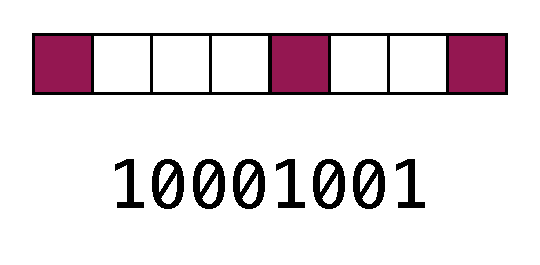
\includegraphics[width=.3\textwidth]{figures/bitmap_bitstring}
\caption{The bitmaps managing the allocated space in a span
  (visualized as allocated objects in the span, top) can be
  represented as bitstrings of 0s and 1s (bottom), where a 1
  corresponds to an allocated object and 0 to free space.}
\label{fig:bitmap-bitstring}
\end{figure}
\end{comment}

This section provides a high-level overview of how \Mesh{} works and
gives some intuition as to how its algorithms and implementation
ensure its efficiency and effectiveness, before diving into detailed
description of \Mesh{}'s algorithms (\S\ref{sec:algorithms}),
implementation (\S\ref{sec:allocator}), and its theoretical analysis
(\S\ref{sec:theory}).


\subsection{Remapping Virtual Pages}

\Mesh{} enables compaction without relocating object addresses; it
depends only on hardware-level virtual memory support, which is
standard on most computing platforms like x86 and ARM64. \Mesh{} works
by finding pairs of pages and merging them together \emph{physically}
but not \emph{virtually}: this merging lets it relinquish
physical pages to the OS.

Meshing is only possible when no objects on the pages occupy the same
offsets.  A key observation is that as fragmentation increases (that
is, as there are more free objects), the likelihood of successfully
finding pairs of pages that mesh also increases.

Figure~\ref{fig:meshing} schematically illustrates the meshing
process. \Mesh{} manages memory at the granularity of \textit{spans},
which are runs of contiguous 4K pages (for purposes of illustration,
the figure shows single-page spans). Each span only contains
same-sized objects. The figure shows two spans of memory with low
utilization (each is under $40\%$ occupied) and whose allocations are at non-overlapping offsets.


\begin{comment}

More formally, we can say that $t$ spans
\textit{\mesh} if and only if the sum of each offset across the $t$
spans sum to 1 or less:

\begin{align}
  \forall k \in [0, b-1]. \sum_{0 \leq i \leq t} s_i[k] \leq 1
\end{align}

where $b$ is span length, and $s_i[k] = 1$ iff there is an object at the $k$th offset of span i.
\end{comment}

Meshing consolidates allocations from each span onto one physical span.
Each object in the resulting meshed span resides at the same offset as
it did in its original span; that is, its virtual addresses are
preserved, making meshing invisible to the application. Meshing then
updates the virtual-to-physical mapping (the page tables) for the
process so that both virtual spans point to the same physical
span. The second physical span is returned to the OS.  When average
occupancy is low, meshing can consolidate many pages, offering the
potential for considerable space savings.
% consolidated to a single span and all other spans can be reused.


\subsection{Random Allocation}

A key threat to meshing is that pages could contain objects at the
same offset, preventing them from being meshed. In the worst case, all
spans would have only one allocated object, each at the same offset,
making them non-meshable. \Mesh{} employs randomized allocation to
make this worst-case behavior exceedingly unlikely. It allocates
objects uniformly at random across all available offsets in a span. As
a result, the probability that all objects will occupy the same offset
is $\left({1}/{b}\right)^{n-1}$, where $b$ is the number of objects in
a span, and $n$ is the number of spans.

%Meshing employs random allocation to minimize the likelihood of this happening too often. The use of a randomized algorithm lets us reason about the effectiveness of meshing in expectation.

%Meshing introduces a limited amount of randomness to ensure that we
%can reason about meshing spans in expectation.

In practice, the resulting probability of being unable to mesh many
pages is vanishingly small. For example, when meshing 64 spans with
one 16-byte object allocated on each (so that the number of objects
$b$ in a 4K span is $256$), the likelihood of being unable to mesh any
of these spans is $10^{-152}$. To put this into perspective, there are
estimated to be roughly $10^{82}$ particles in the universe.

We use randomness to guide the design of \Mesh{}'s algorithms
(\S\ref{sec:algorithms}) and implementation (\S\ref{sec:allocator});
this randomization lets us prove robust guarantees of its performance
(\S\ref{sec:theory}), showing that \Mesh{} breaks the Robson bounds with
high probability.

% ,
%subject to an assumption that application allocation behavior does not
%depend on the addresses returned by the allocator.

%% TODO: should insert a treatment of Emery's ideas about address obliviousness somewhere.


\subsection{Finding Spans to Mesh}

Given a set of spans, our goal is to mesh them in a way that frees as
many physical pages as possible. We can think of this task as that of
partitioning the spans into subsets such that the spans in each subset
mesh. An optimal partition would minimize the number of such subsets.

%% TODO: fix ref to point at exact subsection in algorithms.

Unfortunately, as we show, optimal meshing is not feasible
(\S\ref{sec:theory}). Instead, the algorithms in
Section~\ref{sec:algorithms} present practical methods for finding
high-quality meshes under real-world time constraints. We show that
solving a simplified version of the problem (\S\ref{sec:algorithms})
is sufficient to achieve reasonable meshes with high probability
(\S\ref{sec:theory}).


\begin{comment}
Memory fragmentation, introduced in Section~\ref{sec:introduction},
occurs when the ratio of program-allocated memory to operating-system
reserved memory becomes high:

\begin{align*}
\text{Fragmentation} = \frac{\text{Reserved}}{\text{Allocated}}
\end{align*}

\end{comment}

%%\textit{XXX: I think it is worth noting that an allocator that stored a very high amount of metadata per allocation (e.g. tracking the   meshability graph explicitly) would be indistinguishable from a   highly-fragmented allocator from the perspective of the OS.  Not   sure how to work that in.}

%% Informally, fragmentation occurs because the application manages
%% memory in bytes, while the operating system manages memory at page
%% granularity -- 4 KiB on most current architectures.  Sparsely allocated
%% application addresses ``pin down'' otherwise vacant OS pages.

%% Many managed languages like Java and JavaScript do not experience
%% memory fragmentation due to the combination of language soundness and
%% garbage collection implementations.  Languages are designed in such a
%% way that implementations can enumerate and update all object
%% references, enabling garbage collectors to periodically compact live
%% objects.  This isn't possible for unmanaged languages like C, C++ and
%% Rust, as it is not possible to soundly enumerate all object
%% references.


%% XXX: we should unify talking about ``objects'' and ``allocations''
%% -- allocations is probably better for unmanaged languages where
%% objects have a specific interpretation.

%% Meshing works on \textit{spans} -- contiguous regions of memory where
%% the size of a span is a multiple of the page size between 4 KiB and
%% 128 KiB.  Each span allocates objects of a single-size only, for
%% example a 4 KiB span might hold 32 objects of size 128 bytes.  We can
%% represent a span by a \textit{bitstring}, as in
%% Figure~\ref{fig:bitmap-bitstring}, a string with a 1 for an allocated
%% object at that offset from the start of the span and 0 otherwise.  The
%% length of the bitstring is the number of objects that span holds.

%% This definition characterizes the constraints of the technique by
%% which meshing is possible, wherein two or more spans are meshed or
%% "stacked" on top of each other.

%% The layout and management of a program's heap guide how we consider
%% meshing.  In a running program, the heap is managed as a number of
%% different \textit{size classes} along with a region consisting of
%% large allocations.  Allocations are fulfilled from the smallest size
%% class they fit in (e.g. an allocation request for 50 bytes is
%% satisfied by the 64-byte size class), and objects larger than 16 KiB
%% are individually served from the large allocation region.

%% We treat each size class as an independent instance of the meshing
%% problem, and large allocations are not meshed.  As large allocations
%% are all many multiples of the page size significant fragmentation
%% between them does not exist.  The number of size-classes is fixed at
%% compilation time and constant during the execution of a program.

%% From here, we consider meshing as dealing with a single size-class,
%% and refer to all spans within this size class as $S$.  If we want to
%% mesh the entire heap, this means solving $n$ instances of the meshing
%% problem, where $n$ is the number of size classes.


%% Finally, meshing relies on the fact that there are two types of spans,
%% virtual and physical.  A \textit{virtual} span refers to the memory
%% addresses visible to the program being executed, while a
%% \textit{physical} span corresponds to the area in memory where
%% allocated objects live.  Meshing is concerned with minimizing the
%% count of in-use physical spans without modifying or moving virtual
%% spans.  As noted in Section~\ref{sec:introduction}, we cannot change
%% or modify virtual addresses returned from the allocator, as we do not
%% have a way to enumerate and update all references the program has
%% stored.  Since the last two digits of a virtual address directly
%% specify the offset of the referenced object in the span, objects
%% cannot be safely relocated to a different offset, leading to our

%% Allocated objects and free space within a span are tracked by the
%% memory allocator as a bitmap (see Section~\ref{sec:allocator}) -- the
%% in-memory representation of a bitstring.  For example, for objects of
%% size 32 and a span size of 4 KiB, the span can hold 128 32-byte
%% objects, so allocated objects are be tracked with a 128-bit bitmap.
%% Each allocated object in a running program has a unique
%% \textit{(bitmap, offset)} tuple.  Bitmaps are between 8 and 256-bits
%% in length.

%% We can therefore think of the meshing problem as that of partitioning
%% a set of equal-length bitstrings such that the bitstrings in each subset
%% mesh.  An optimal partition would minimize the number of such subsets.
%% This abstraction allows us to analyze the complexity of this computational
%% task in Section~\ref{sec:theory}.
